\chapter{Context survey}
\section{Context}

The University of St.\ Andrews' School of Computer Science originally had a class size of approximately 30 students. It has had a relatively rapid expansion, with class size of over 200 students. Although the student to staff ratio has remained fairly consistent (somewhere between 30 and 20 to 1) throughout the years, the logistics of class management became more difficult. Educators have becoming aware of this increasing need for an alternative solution.

Moving to online learning in the wake of the global pandemic, the need for an alternative became immediate. The school developed a system for managing online labs using Microsoft Teams \cite{teams}, adapting it in a fairly expedient manner. The current system meets the basic needs for managing online labs, however is lacking in a few key areas.  

The School of Computer Science requires a system for managing labs that meets its specific needs. The system should enable class demonstrators to assist in the resolution of problems students have, should enable lab leads to review labs and address some of the specific nuances that the domain requires - for example addressing the lab opening times. A single application should meet these needs so that the system is easy to use, adapt and maintain.

There are some existing categories of application which could meet the above needs. A small number of classroom management tools exist. Another, much more common, type of application are incident management tools - often used for tracking and logging IT incidents and problems. Both types of application shall be considered and evaluated in order to gain insight into their suitability.
 
This section shall discuss and review two common examples of these types of application, as well as the current system used by the school.

\section{Current System}

The current system for managing online lab sessions was developed and adapted at short notice due to the global pandemic. The initial solution was to create a `CS1000 Labs' team on Microsoft Teams \cite{teams}, the University's standard collaboration tool for online learning, and manage the lab sessions by posting announcements when labs opened. Students were then able to post new conversations under these announcements, which prompted them to tag the class demonstrators, and briefly summarising their issue and provide module code and practical number associated with their issue.

TODO: power automate flows owned by system admin, in control of them/nobody else can access them,
TODO collaboration students lost, cheating
TODO: maintenance locations, complicated sharepoint/automate

\FloatBarrier
\begin{figure}[H]
  \centering
  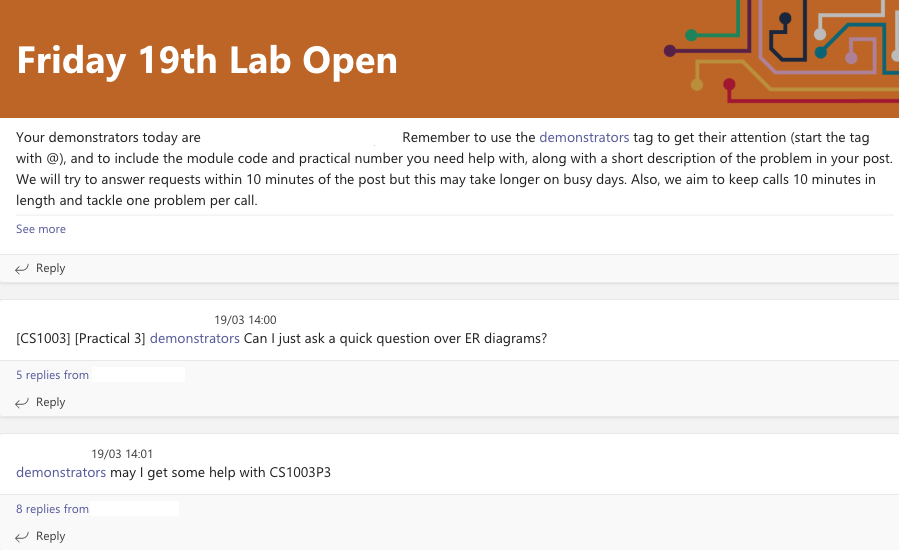
\includegraphics[width=section\textwidth]{2literature/images/teams1.png}
  \caption{An example of the first iteration process of managing online labs.}
\end{figure}

The second, and current, iteration of the current system uses a form input. This is accessed using a `Request Form' tab in the Microsoft Teams \cite{teams} CS1000 Labs team. 

\FloatBarrier
\begin{figure}[H]
  \centering
  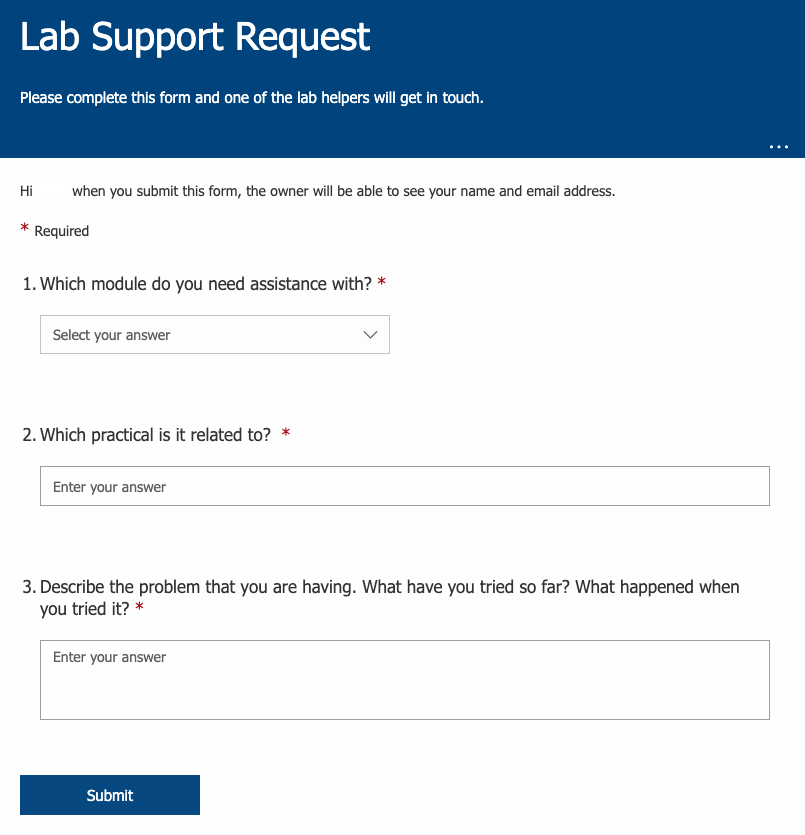
\includegraphics[width=0.85section\textwidth]{2literature/images/teams2a.png}
  \caption{The request form from the second iteration process of managing online labs.}
\end{figure}

The form uses Power Automate \cite{pauto} to post on a private demonstrator team channel (used only to create a notification for class demonstrators) and add the form data to a Microsoft List \cite{lists}.

\FloatBarrier
\begin{figure}[H]
  \centering
  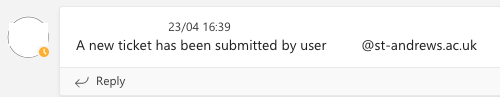
\includegraphics[width=0.6section\textwidth]{2literature/images/teams2b.png}
  \caption{The format of posts on the private demonstrator channel used to create notifications.}
\end{figure}

On this real-time collaborative spreadsheet, class demonstrators can assign themselves to students' requests before they make contact with the student through Microsoft Teams \cite{teams} or email. 

TODO notes:
\begin{itemize}
  \item communication in video or text (depending on issue complexity) but both on teams
\end{itemize}

\FloatBarrier
\begin{figure}[H]
  \centering
  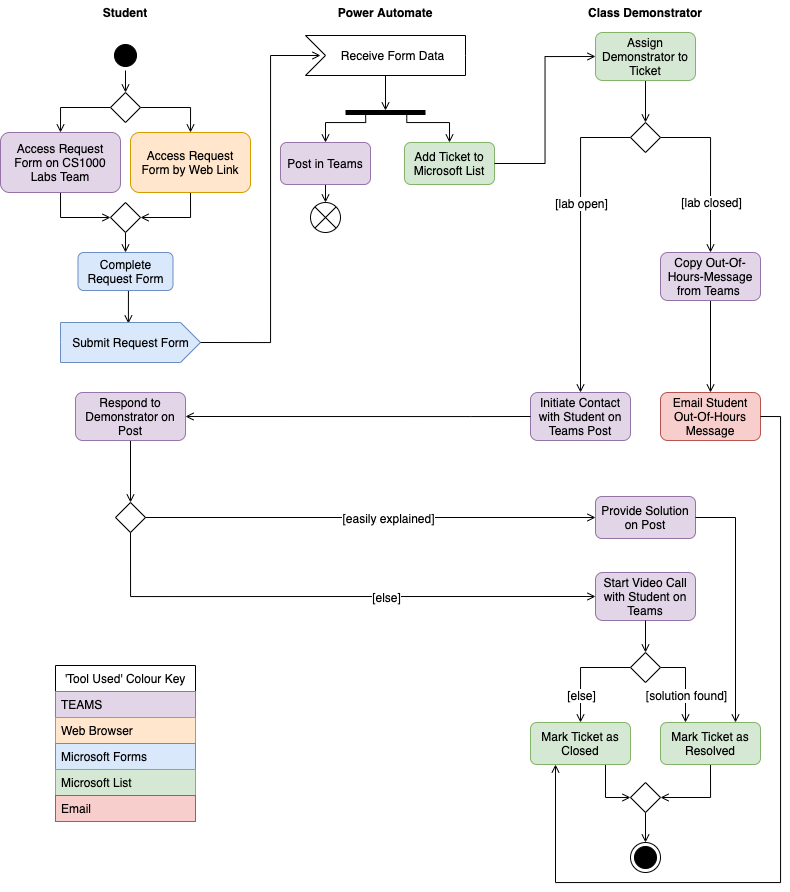
\includegraphics[width=section\textwidth]{2literature/images/activityRevised.png}
  \caption{Activity diagram for existing method of managing student online lab request.}
\end{figure}

\subsection{Software Evaluation}

\paragraph{Accessibility}
The current system meets the end user basic needs reasonably well. As a result of its integration with Microsoft Teams \cite{teams}, the form and navigation to it meet standard accessibility requirements \cite{formaccess} \cite{teamsaccess}. TODO worth mentioning this ? should this be a category?


\paragraph{Functionality}
For students, the functionality of the software is adequate. The form provides a method of posting issues to demonstrators. However, there are some further areas of functionality that the current system fails. The form does not given any indication of how busy the current lab is. Also, there are no means to withdraw a form from the demonstrators' Microsoft List after posting. Further, the lab form allows students to post tickets outwith lab hours, meaning that they may wait some time (expecting a solution) before receiving a manual response about the lab being closed. Additionally, there is no simple way to access the help that other students received for similar issues - although an FAQ tab exists in Microsoft Teams \cite{teams}, it requires manual recognition of common problems and updating, meaning that the amount of solutions collected is significantly lower than with an automated system. 
        
For class demonstrators, the functionality is fairly adequate. The Microsoft List contains information on posted student issues, with the bonus of real-time updates from other demonstrators. There are functionality pitfalls for demonstrators too. One comes from the fact that the request form does not require much information about the problem, for example a minimum length of description or issue category, meaning that demonstrators do not have a lot of information before speaking to the student. Also, there is no functionality regarding lab opening hours - meaning that demonstrators must manually reply to all requests posted outwith lab hours.

For lab leads, there is no additional functionality. Lab leads must manually analyse the Microsoft List or Microsoft Teams \cite{teams} channel in order to gain further information. 

\paragraph{Performance}  
When used correctly by both class demonstrators and students, the system performs basic functionality well. The issue with the system is that it consists of multiple communicating platforms, however each platform is owned and maintained to a high standard by Microsoft. Performance issues could arise if applications were to be updated.

\paragraph{Ease of Use} 
For students, the system is fairly self explanatory and easy to use. Students simply access the form, provide information and then wait to be contacted by class demonstrators.

For class demonstrators, the system is more difficult to use. Since the system is comprised of multiple platforms, each must be considered when running a lab. For example, the demonstrators are notified of a new issue in Microsoft Teams \cite{teams}, the issue ticket is located in a Microsoft List spreadsheet and then communication with the student must be carried out in teams and/or email. It is worth nothing that the increased number of platforms increase the surface area for human error.


\paragraph{Customisation} 
Customisation in this system is reasonable. The form input fields and therefore the Microsoft List spreadsheet labels are customisable. The power automate \cite{pauto} flows (non-code scripts) are also customisable, however only within the limits of Microsoft's provided actions and applications.

\paragraph{Compatibility}  
The form is located in teams, along with the spreadsheet of issues for demonstrators. Communication is also carried out mostly using either the comment or video call features within Microsoft Teams. Since Microsoft Teams is the University wide standard collaboration tool for online learning, and is integrated with the University's Shibboleth \cite{shib} single sign-on platform, students should already have the technology installed and working on their machines. Additionally, the Microsoft Teams mobile application and form enable students to easily post tickets from their mobile devices.

TODO: cite teams every time ???

\paragraph{Robustness}
Robustness is where the current system fails. As discussed previously and conveyed in the activity diagram, the system is comprised of multiple, interlinked applications as well as manual input. If any of the applications are updated, down or behaving in an unexpected way then the system could fail to function - this could be difficult to detect in quieter labs and result in students waiting indefinitely on a response.


\paragraph{Cost}  
The current system is not free, however is covered by existing Microsoft Office licensing purchased by the university.  


\newpage
\section{Classroom Management Tools}

ClassroomQ is a good example of existing classroom management tools. It offers a very simple system, where teachers can create a classroom which students can join, type a message and hit an `Assistance Needed' button to join the queue of students who need help. The basic process is shown below.

Firstly, the teachers start a classroom session.

\FloatBarrier
\begin{figure}[H]
  \centering
  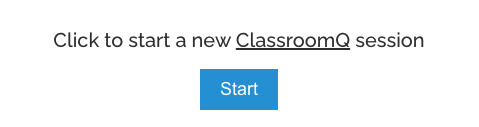
\includegraphics[width=0.5section\textwidth]{2literature/images/cq1.png}
  \caption{Teacher's screen when a class has not been started.}
\end{figure}

The classroom is created, showing the class code which students can use to join.

\FloatBarrier
\begin{figure}[H]
  \centering
  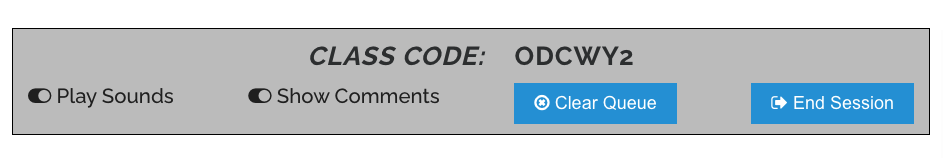
\includegraphics[width=0.75section\textwidth]{2literature/images/cq2.png}
  \caption{Real time classroom queue, showing class join code and current requests.}
\end{figure}

Students join by entering their name and class code.

\FloatBarrier
\begin{figure}[H]
  \centering
  
\includegraphics[width=0.5section\textwidth]{2literature/images/cq3.png}
  \caption{Student join page, showing sample class code and name.}
\end{figure}

Below is the image shown to students once they have joined the class. From this page they are able to type details of their problem in the comment section and then click the `Assistance Needed' button to join the queue.

\FloatBarrier
\begin{figure}[H]
  \centering
  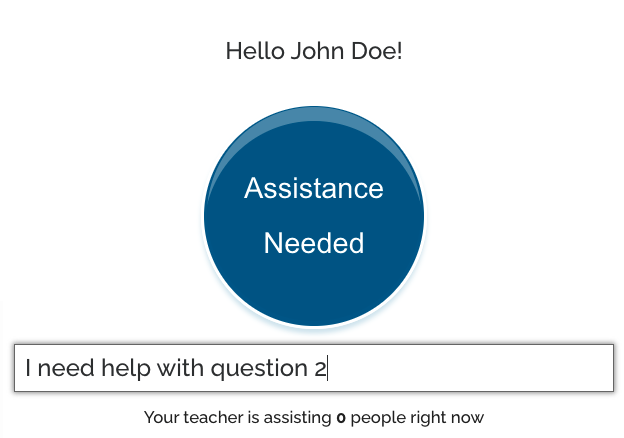
\includegraphics[width=0.5section\textwidth]{2literature/images/cq4.png}
  \caption{Student help request page.}
\end{figure}

Once the student has joined the queue, they are taken to the page below. This allows them to cancel their request as well as providing real time information about their position in the queue.

\FloatBarrier
\begin{figure}[H]
  \centering
  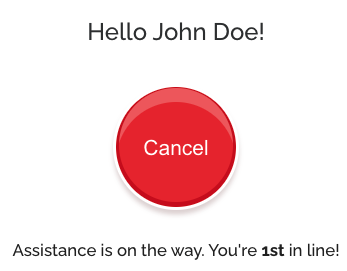
\includegraphics[width=0.5section\textwidth]{2literature/images/cq5.png}
  \caption{Student page after posting help request.}
\end{figure}

The teacher is then able to see an ordered view of the student's requests in on the class page.

\FloatBarrier
\begin{figure}[H]
  \centering
  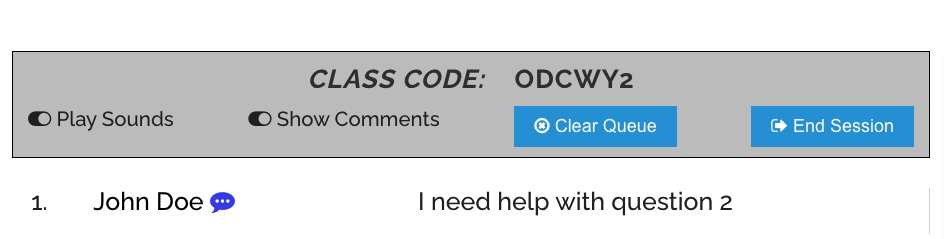
\includegraphics[width=0.75section\textwidth]{2literature/images/cq6.png}
  \caption{Teacher's class page view after the request has been posted.}
\end{figure}


\subsection{Software Evaluation}

\paragraph{Functionality}
The website provides similar functionality to what we require in terms of being able to post issues, however is not suitable for a number of reasons.

For students, the amount of information they can provide is extremely limited. Only a single comment box, with a maximum of 190 characters, is available and therefore restricts students from providing a detailed description of their issue. There is also no prompt for any class or issue category information. Students are also unable to have more than one live request at a time. It is useful for all parties that the class sessions can be ended - stopping requests for help being posted outwith lab hours.

For class demonstrators, only a single account can be used - the system does not allow classes to have multiple teachers. This alone makes the application unsuitable, since there is no way to organise which demonstrator is assigned to which task. The system does not contain any integrated communication methods of any type. The system's method of obtaining student names is also unsuitable for managing school labs, since students could provide any form of name - something that would introduce issues when attempting to communicate with the student on a different system. Teacher accounts are also only able to, forever, open a single class with a persistent class code, meaning that running multiple labs or different labs is not possible.

For lab leads, no functionality exists that is separate from class demonstrators. However, it is possible to export logs of students who joined, as well as their help requests, which could be analysed in another platform.


\paragraph{Performance}  
It is hard to give an assessment of the system without it having been used in class. However, the application is fairly lightweight and has simple functionality so it is hard to foresee performance issues. TODO worth keeping this in?

\paragraph{Ease of Use}
The system's simplicity makes it extremely easy and intuitive to use. It is also possible to use the application on mobile. 

It is worth noting that for use in managing the University labs, this software would require communication on a different platform. Since the application does not enforce, or allow the enforcement of, validation of names, it would be difficult to find students on third party applications.


\paragraph{Customisation} 
The application provides no options for customisation of any kind.


\paragraph{Compatibility}  
Being web based means that students are not required to download and install any third-party software. 


\paragraph{Robustness}
As with performance, it is hard to give an assessment of the system without it having been used in class. It is, again, reasonable to expect that the application is fairly robust given its simplicity.


\paragraph{Cost}  
The system offers multiple membership levels which cost varying amounts. The level that would be required for the University of St.\ Andrews would be \$12.99 per year per teacher, for a minimum of 5 teacher accounts.


\newpage
\section{Incident Management Tools}

Spiceworks Cloud Help Desk is a good example of existing incident management tools. It is a free to use, cloud-based help desk that is used by IT professionals. Traditionally, the system is used to track and manage IT issues in order to provide IT support, however the system could also be used to track and manage requests for help in our lab management domain. The basic process is shown below.

Firstly, students would access a link to the help portal and enter their email address.

\FloatBarrier
\begin{figure}[H]
  \centering
  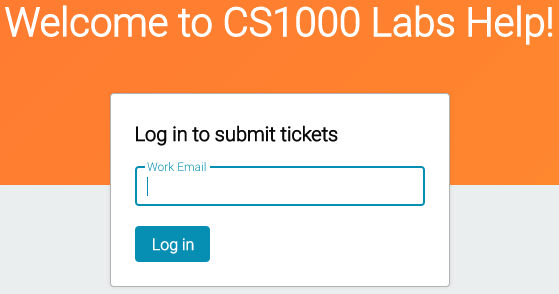
\includegraphics[width=0.5section\textwidth]{2literature/images/SWportalLogin.png}
  \caption{Login screen from portal link.}
\end{figure}

The student would then, if authorised, receive an email link to login to the portal. This would take them to the following form.

\FloatBarrier
\begin{figure}[H]
  \centering
  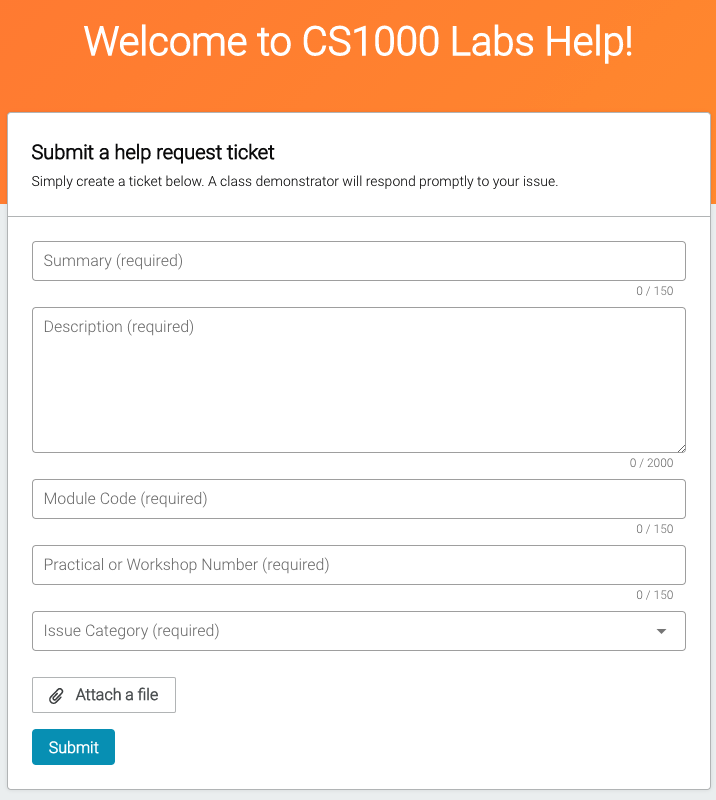
\includegraphics[width=0.65section\textwidth]{2literature/images/SWpostTicket.png}
  \caption{Ticket posting form, reached after login.}
\end{figure}

The ticket would then appear on the class demonstrator help desk.

\FloatBarrier
\begin{figure}[H]
  \centering
  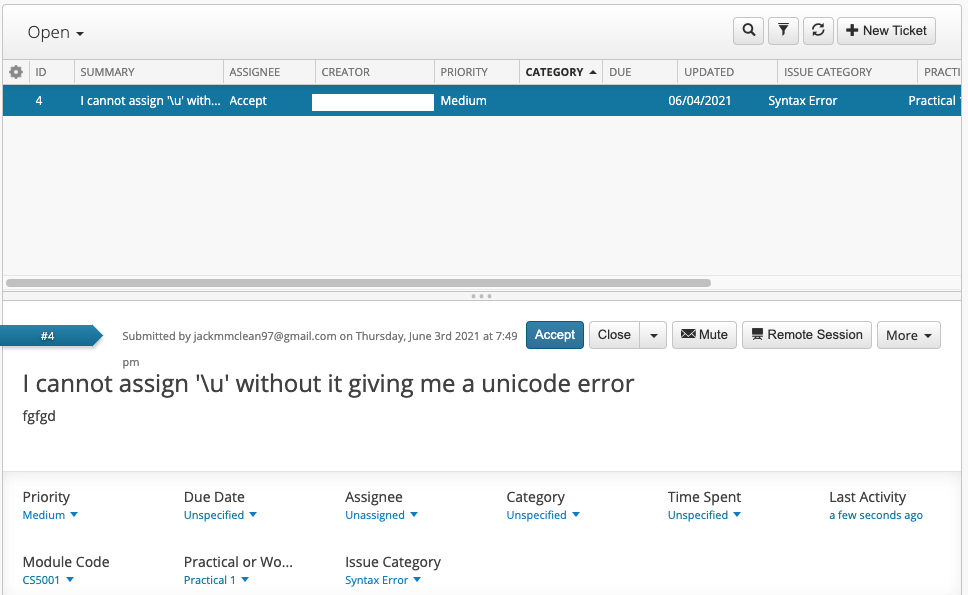
\includegraphics[width=0.85section\textwidth]{2literature/images/SWticketPage.png}
  \caption{The help desk ticket page, accessible to class demonstrators.}
\end{figure}

Class demonstrators are then able to respond to the ticket on Spiceworks, notifying the user by email, and initiate a video call on a different service if necessary. The demonstrator can then close the ticket when complete.

\subsection{Software Evaluation}

\paragraph{Functionality}
For students, spiceworks is functional to the point that we require for our system. The system allows tickets to be created via a customisable user portal, which can be modified to include module code, practical number and issue category in text field, text area and select inputs. The system also allows tickets to be posted by email. One issue with functionality is that some attributes are `baked-in' to the system, for example it is not possible to remove the `summary' or `description' input fields from the ticket posting form. Additionally, the system has a due date attribute for tickets that cannot be removed.

For class demonstrators, the ticket management UI functions well. It allows tickets to be assigned, edited, closed, merged with other tickets. The system also has a useful `last activity' attribute on each ticket. The privacy controls on the user portal also allow an `active directory' to be created, something that would be useful in authenticating to ensure users are students. A timeline feature on the system also shows demonstrators a time sorted list of all activities. There is no way to distinguish between tickets that have been resolved or closed unsuccessfully. 

For lab demonstrators, a useful summary dashboard is provided. This provides useful infographs and key statistics such as average first response time, average ticket close time, ticket category breakdown and top ticket creators. It does not provide any information on specific class demonstrators, however Spiceworks allows the generation of summary reports which can be produced for each individual demonstrator. The system also does not have any option to prevent tickets being posted outwith lab hours, although this information could be added to an autmatic email response. It is also important to note that there are no different admin roles on Spiceworks - functionality does not differ between class demonstrators and lab leads.


\paragraph{Performance}
As with ClassroomQ, it is hard to comment on the domain specific performance. However, Spiceworks is an established, popular ticketing system and therefore a reasonable level of performance would be expected. 


\paragraph{Ease of Use} 

The system is fairly simple and intuitive to use for students. The administrative aspect is slightly more complex, however would be quick and easy to learn after the initial setup. One issue is that the system is designed for tech issue ticketing, therefore some of the application and documentation language refers specifically to that domain.

\paragraph{Customisation} 

The system is fairly customisable. It also different form attributes to be added to the user portal, therefore also to the tickets. There is no option to customise other aspects of the system, such as the summary dashboard


\paragraph{Compatibility}  

This system has the advantage of being web based, meaning that users do not need to download and install third party content. It is also possible to import and export tickets in JSON form, meaning that tickets could be easily migrated to or from the system.

\paragraph{Robustness}
As with performance, it is hard to give an assessment of the system without it having been used in class. It is, again, reasonable to expect that the application is fairly robust given its popularity.


\paragraph{Cost}  
All Spiceworks products are entirely free. They are, however, funded by advertising revenue which is generated by selling data stored on Spiceworks. This could be a serious issue for the lab management domain, as students would be well within their right to refuse the service. Another problem is that Spiceworks terms of use specifies that organisations must obtain permission to use the service.
